\begin{figure}
  \begin{tabular}{cc}
    \begin{minipage}{0.5\hsize}
      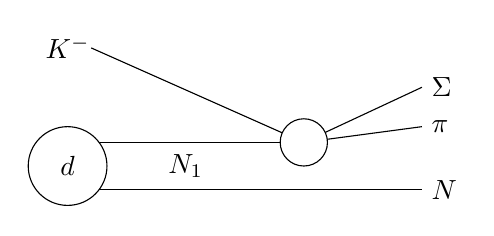
\begin{tikzpicture}
        \draw (0.0, 1.5) node {$K^-$};
        \draw (0.3, 1.5)-- (3, 0.3);      
        \draw (0,  0.3) -- (3,  0.3);
        \draw (0, -0.3) -- (4.5, -0.3) [right] node{$N$};
        \draw (3,  0.3) -- (4.5, 0.5) [right] node{$\pi$};
        \draw (3,  0.3) -- (4.5, 1.0) [right] node{$\Sigma$};
        
        \draw [fill=white](3, 0.3) circle (0.3);
        \draw [fill=white](0, 0) circle (0.5) node{$d$};

        \draw node at (1.5, 0.0){$N_1$};
      \end{tikzpicture}
    \end{minipage}
    
    \begin{minipage}{0.5\hsize}
      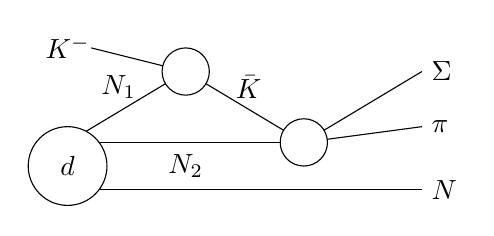
\begin{tikzpicture}
        \draw (0.0, 1.5) node {$K^-$};
        \draw (0.3, 1.5)-- (1.5, 1.2);
        \draw (0,  0.3) -- (3,  0.3);
        \draw (0, -0.3) -- (4.5, -0.3) [right] node{$N$};
        \draw (3,  0.3) -- (4.5, 0.5) [right] node{$\pi$};
        \draw (3,  0.3) -- (4.5, 1.2) [right] node{$\Sigma$};

        \draw (1.5, 1.2)-- (3.0, 0.3);
        \draw (0.0, 0.3)-- (1.5, 1.2);      
        \draw [fill=white](1.5, 1.2) circle (0.3);
        \draw [fill=white](3.0, 0.3) circle (0.3);
        \draw [fill=white](0, 0) circle (0.5) node{$d$};

        \draw node at (2.3, 1.0){$\bar{K}$};
        \draw node at (0.65, 1.0){$N_1$};
        \draw node at (1.5, 0.0){$N_2$};
      \end{tikzpicture}
    \end{minipage}
  \end{tabular}
  \caption{
    Fynman diagrams about $d(K^-, N)"\pi\Sigma"$ reaction.
    The left and right figures indicate about 1-step and 2-step reactions, respectively.
  }
  \label{fig:kd_diag}
\end{figure}
